\documentclass[10pt]{beamer}
\usetheme[
%%% options passed to the outer theme
%    hidetitle,           % hide the (short) title in the sidebar
%    hideauthor,          % hide the (short) author in the sidebar
%    hideinstitute,       % hide the (short) institute in the bottom of the sidebar
%    shownavsym,          % show the navigation symbols
%    width=2cm,           % width of the sidebar (default is 2 cm)
%    hideothersubsections,% hide all subsections but the subsections in the current section
%    hideallsubsections,  % hide all subsections
%    left                % right of left position of sidebar (default is right)
  ]{Aalborg}
  
% If you want to change the colors of the various elements in the theme, edit and uncomment the following lines
% Change the bar and sidebar colors:
%\setbeamercolor{Aalborg}{fg=green!20,bg=green}
%\setbeamercolor{sidebar}{bg=red!20}
% Change the color of the structural elements:
%\setbeamercolor{structure}{fg=red,bg=red!10}
% Change the frame title text color:
%\setbeamercolor{frametitle}{fg=blue,bg=red}
% Change the normal text color background:
%\setbeamercolor{normal text}{bg=gray!10}
% ... and you can of course change a lot more - see the beamer user manual.

\usepackage[utf8]{inputenc}
\usepackage[spanish]{babel}
%\usepackage[T1]{fontenc}
% Or whatever. Note that the encoding and the font should match. If T1
% does not look nice, try deleting the line with the fontenc.
\usepackage{helvet}
\usepackage[compatibility=false]{caption}
\usepackage{subcaption}
\usepackage{multicol}
\usepackage{hyperref}
\usepackage{textcomp}
\usepackage{gensymb}
\usepackage{verbatim}

% colored hyperlinks
\newcommand{\chref}[2]{%
  \href{#1}{{\usebeamercolor[bg]{Aalborg}#2}}%
}

\title[Introducción a \LaTeX]% optional, use only with long paper titles
{Introducción a \LaTeX}

\subtitle{Clase 1}  % could also be a conference name

\date{\today}

\author[Jhabriel Varela, Ch.E.] % optional, use only with lots of authors
{
  Jhabriel Varela, Ch.E. \\
  \href{mailto:jhabriel.varela@upa.edu.py}{{\tt jhabriel.varela@upa.edu.py}}
}
% - Give the names in the same order as they appear in the paper.
% - Use the \inst{?} command only if the authors have different
%   affiliation. See the beamer manual for an example

\institute[
%  {\includegraphics[scale=0.2]{aau_segl}}\\ %insert a company, department or university logo
  UPA\\
  Paraguay
] % optional - is placed in the bottom of the sidebar on every slide
{% is placed on the bottom of the title page
  Universidad Paraguayo-Alemana\\
  Paraguay
  
  %there must be an empty line above this line - otherwise some unwanted space is added between the university and the country (I do not know why;( )
}

% specify the logo in the top right/left of the slide
\pgfdeclareimage[height=.8cm]{mainlogo}{figures/UPA_JPG} % placed in the upper left/right corner
\logo{\pgfuseimage{mainlogo}}

% specify a logo on the titlepage (you can specify additional logos an include them in 
% institute command below
\pgfdeclareimage[height=1.3 cm]{titlepagelogo}{figures/UPA_JPG} % placed on the title page
%\pgfdeclareimage[height=1.5cm]{titlepagelogo2}{AAUgraphics/aau_logo_new} % placed on the title page
\titlegraphic{% is placed on the bottom of the title page
  \pgfuseimage{titlepagelogo}
%  \hspace{1cm}\pgfuseimage{titlepagelogo2}
}

\begin{document}
% LA PORTADA
{\aauwavesbg
\begin{frame}[plain,noframenumbering] % the plain option removes the sidebar and header from the title page
  \titlepage
\end{frame}}
%%%%%%%%%%%%%%%%

% TABLA DE CONTENDIDOS
\begin{frame}{Contenido}{}
\tableofcontents
\end{frame}
%%%%%%%%%%%%%%%%

\section{Generalidades}
% Generalidades del Tex
\begin{frame}{Generalidades}
	\begin{block}{¿Qué es \TeX ?}
		Es un programa de ordenador creado por Donald E. Knuth. Es ampliamente utilizado para componer textos y fórmulas matemáticas.
	\end{block}
	\begin{block}{¿Qué es \LaTeX{}?}
	\LaTeX{} es un paquete de macros que permite a los autores componer e imprimir su trabajo con la mayor calidad tipográfica, usando un formato profesional predifinido. Fue escrito por Leslie Lamport. Emplea el formateador \TeX{} como motor de composición.
	\end{block}
	\begin{alertblock}{¿Cómo se pronuncia?}
		\TeX{} se pronuncia “tej''. La “j” surge del alfabeto griego donde X es la letra “j” o “ji”. \LaTeX{} se pronuncia “Látej”.
	\end{alertblock}	
\end{frame}
%%%%%%%%%%%%%%%%

% ¿Cómo funciona?
%\begin{frame}{Generalidades}
%	\begin{block}{¿Cómo funciona?}
%	Generalmente, a la hora de publicar un texto, el \emph{autor} envía su manuscrito a la editorial. El \emph{maquetador} decide el aspecto del documento (anchura de columnas, tipografía, espacios,...). El maquetador manda estas instrucciones al \emph{compositor}, quien compone el libro de acuerdo a tales instrucciones.
%	
%	En un entorno \LaTeX{}, \LaTeX{} representa el papel del maquetador y usa \TeX{} como su compositor. Pero \LaTeX{} es sólo un programa y por tanto necesita que el autor proporcione información para describir la estructura lóqica de su trabajo. Estas informaciones se conocen como “órdenes \LaTeX{}”.
%	\end{block}
%\end{frame}

% Producción de textos estructurados
\begin{frame}{Generalidades}
	\begin{block}{Producción de textos estructurados.}
	\vspace{-.4cm}
	\begin{multicols}{2}
		\begin{figure}
			\centering
			\begin{subfigure}[b]{0.5\textwidth} 
				\centering
				
\includegraphics[scale=.04]{figures/autor}
				\caption{El autor}			
			\end{subfigure}
			
			\vspace*{.25cm}			
			
			\begin{subfigure}[b]{0.5\textwidth} 
				\centering
				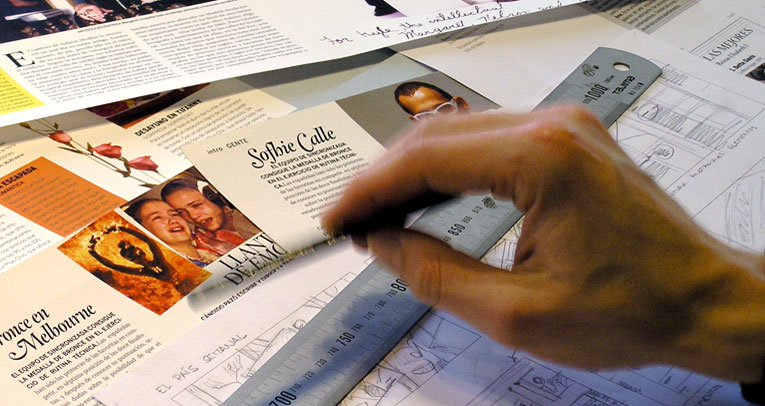
\includegraphics[scale=.08]{figures/maquetador}
				\caption{El maquetador}
			\end{subfigure}
			
			\vspace*{.25cm}				
			
			\begin{subfigure}[b]{0.5\textwidth} 
				\centering
				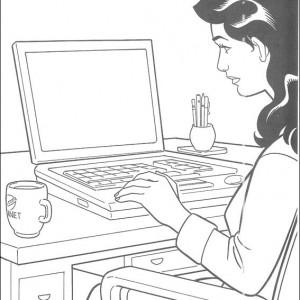
\includegraphics[scale=.12]{figures/compositor}
				\caption{El compositor}
			\end{subfigure}
		\end{figure}	
\newpage

\vspace*{.50cm}
$\rightarrow$ envía su manuscrito a la editorial (al maquetador). 

\vspace*{.70cm}
$\rightarrow$ recibe el manuscrito del autor y decide el aspecto del documento y envía instrucciones al compositor.

\vspace*{.50cm}
$\rightarrow$ recibe las instrucciones del maquetador y compone el libro en base a tales instrucciones.
\end{multicols}
	\end{block}
\end{frame}
%%%%%%%%%%%%%%%%

%Producción de textos estructurados con LaTeX
\begin{frame}{Generalidades}
	\begin{block}{Producción de textos estructurados en \LaTeX{}.}
	\vspace{-.4cm}
	\begin{multicols}{2}
		\begin{figure}
			\centering
			\begin{subfigure}[b]{0.5\textwidth} 
				\centering
				
\includegraphics[scale=.08]{figures/autor_LaTeX}
				\caption{El autor}			
			\end{subfigure}
			
			\vspace*{.25cm}			
			
			\begin{subfigure}[b]{0.5\textwidth} 
				\centering
				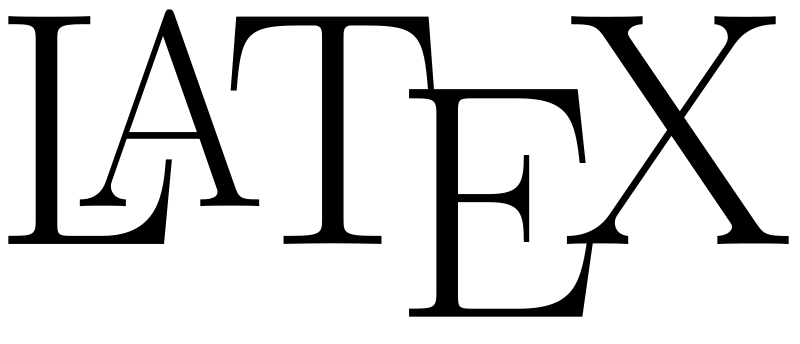
\includegraphics[scale=.09]{figures/maquetador_LaTeX}
				\caption{El maquetador}
			\end{subfigure}
			
			\vspace*{.25cm}				
			
			\begin{subfigure}[b]{0.5\textwidth} 
				\centering
				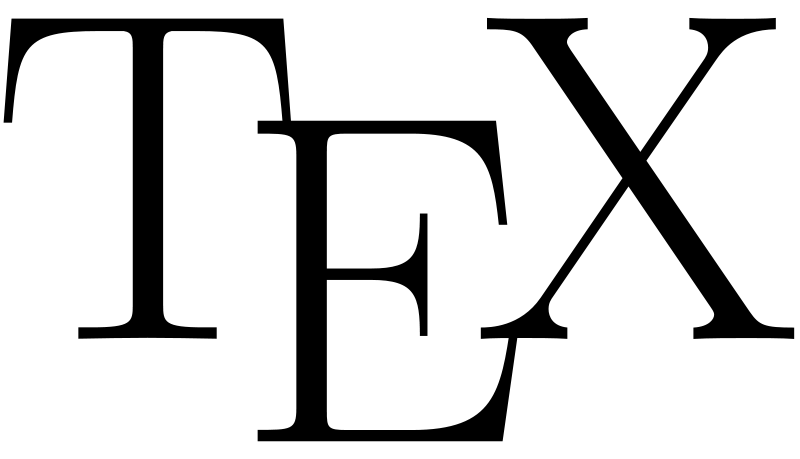
\includegraphics[scale=.06]{figures/compositor_LaTeX}
				\caption{El compositor}
			\end{subfigure}
		\end{figure}	
\newpage

\vspace*{.05cm}
$\rightarrow$ Escribe el texto y \textbf{proporciona información para describir la estructura lógica de su trabajo}.


\vspace*{.70cm}
$\rightarrow$ interpreta la información proveída por el autor y envía las directrices al compositor.

\vspace*{.90cm}
$\rightarrow$ recibe las instrucciones de \LaTeX{} y compone el libro.
\end{multicols}
	\end{block}
\end{frame}
%%%%%%%%%%%%%%%%

\begin{frame}{Generalidades}

\begin{block}{¿Vale la pena tanto esfuerzo?}
	\begin{multicols}{2}
	
	\begin{footnotesize}
	\begin{block}{Ventajas}
		\begin{itemize}
			\item Resultados profesionales.
			\item Amplio soporte para fórmulas matemáticas.
			\item Casi nunca debemos preocuparnos por el aspecto real del documento.
			\item Fácil generar notas de pie, referencias, índices, listas de figuras, tablas de contenido, nomenclaturas, etc.
			\item Amplia gama de paquetes que se ajustan a necesidades específicas.
			\item ¡Es gratis!
		\end{itemize}
	\end{block}			
	\end{footnotesize}

	\newpage	
	
	\begin{footnotesize}
	\begin{block}{Desventajas}
		\begin{itemize}
		\item Esfuerzo y dedicación inicial elevados.
		\item Lo que se escribe en la pantalla no es lo que se ve como resultado. No es un editor de texto del tipo \textbf{WYSIWYG}.
		\item Para los usuarios novatos los errores son habituales, esto suele llevar a que se sientan frustrados.
		\item Aunque existe flexibilidad en el ajuste de parámetros, el diseño de una nueva composición es muy costosa.
		\end{itemize}
		\end{block}
	\end{footnotesize}
	\end{multicols}
\end{block}

\end{frame}

\begin{frame}{Generalidades}
	\begin{block}{\LaTeX{} vs MS Word}
		\begin{figure}
			\centering
			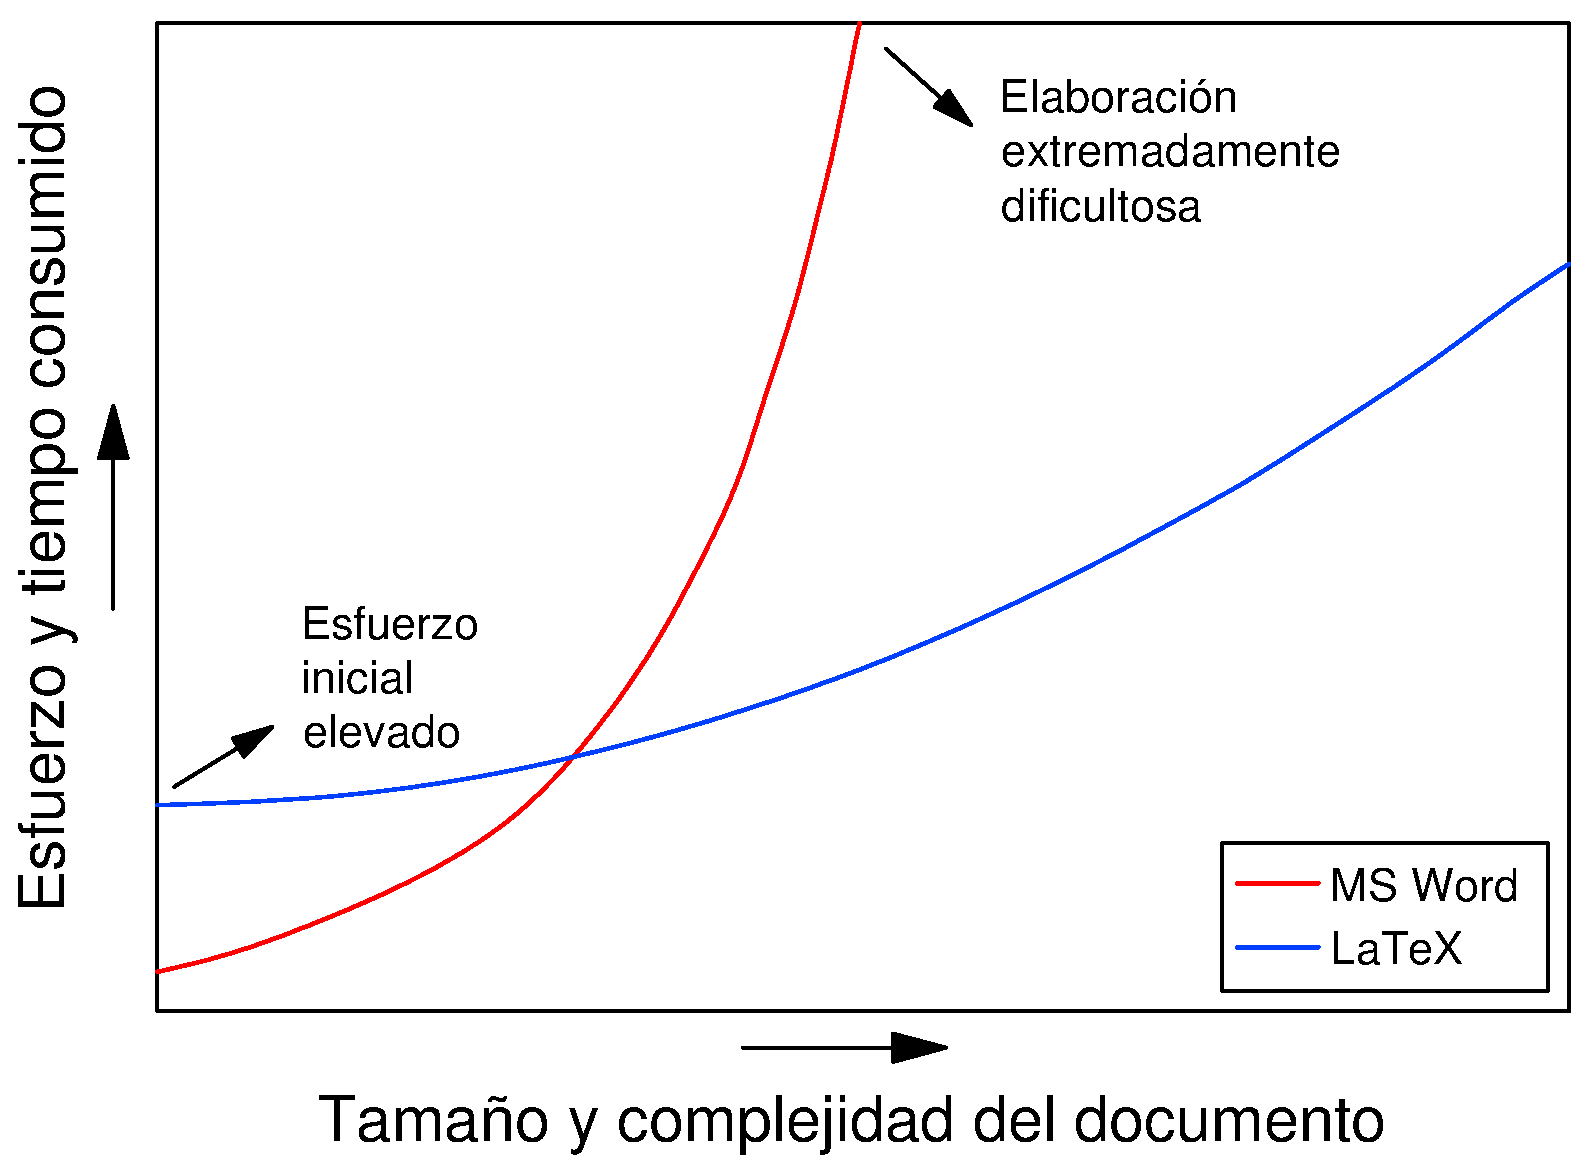
\includegraphics[scale=.3]{figures/LaTeX_vs_Word.pdf}
			\caption{\LaTeX{} vs MS Word}
		\end{figure}
%	\begin{center}
%		¡\LaTeX{} no es para todos, pero podría ser para vos!
%	\end{center}
	\end{block}
\end{frame}
%%%%%%%%%%%%%%%%

\section{Instalación}
\begin{frame}{Instalación y configuración}
	\begin{block}{Guía de instalación}
\href{https://www.dropbox.com/s/8re9ororf9i42et/guia_latex.pdf}{Descargar guía de instalación}
	\end{block}
\end{frame}
%%%%%%%%%%%%%%%%

%% general installation instructions
%\begin{frame}{Instalación en Windows}
%	\begin{block}{Descarga de archivos necesarios}
%		\begin{itemize}
%			\item \textbf{MikTeX:} Es el motor de \LaTeX{} para Windows. Lo podemos descargar \href{http://www.miktex.org/download}{\textbf{aquí}}. Descargar la versión 32 o 64 bits según corresponda.
%			\item \textbf{Ghost View y GhostScript}: Son programas para la visualización de documentos PostScript (formato parecido al PDF). Podemos descargar el Ghost View \href{http://pages.cs.wisc.edu/~ghost/gsview/get50.htm}{\textbf{aquí}} y el GhostScript de  \href{http://sourceforge.net/projects/ghostscript/files/
%			GPL\%20Ghostscript/}	{\textbf{aquí}}. La versión más nueva es la 9.10 (Descargar la versión 32 o 64 bits según corresponda).
%			\item \textbf{TeXMaker:} Es el editor de texto, tiene una interfaz gráfica muy amigable para visualizar bloques, comandos y previsualización de pdf's. Lo podemos descargar \href{http://www.xm1math.net/texmaker/download.html}{\textbf{aquí}}.
%		\end{itemize}
%Una explicación detallada del proceso de instalación puede encontrarse \href{http://conocimientoadictivo.blogspot.com/2011/08/instalar-latex-en-windows.html}{\textbf{aquí}}.
%	\end{block}
%\end{frame}
%%%%%%%%%%%%%%%%%
%
%\begin{frame}{Instalación en Windows}
%	\begin{block}{Instalación de MikTeX}
%		\begin{enumerate}
%			\item Ejecutar el instalador de MikTeX como \textbf{administrador}.
%			\item Aceptar las condiciones de uso e “Instalar para todos los usuarios de este equipo”.
%			\item En \textit{Settings}, seleccionamos A4 como “Preferred paper” y en “Install missing packages” on-the-fly ponemos Yes (MikTex instalará los paquetes faltantes sólo cuando se los invoca).
%			\item El proceso de instalación tarda un par de minutos.
%		\end{enumerate}
%	\end{block}
%
%	Ahora debemos actualizar la base de datos de los paquetes. Vamos a \texttt{Inicio »» Todos los programas »» MikTeX 2.9 »» Maintenance(Admin) »» Settings(Admin)}. En Win8 presionamos \texttt{Win + Q} y en el buscador escribimos \texttt{Settings(Admin)}. Hacemos click en \texttt{Refresh FNDB} y \texttt{Update Formats}.
%\end{frame}
%%%%%%%%%%%%%%%%
%
%\begin{frame}{Instalación en Windows}
%	\begin{block}{Instalación de GhostScript y Ghost View}
%		\begin{enumerate}
%			\item Instalemos primero el GhostScript (Recuerda instalar como Administrador)
%			\item Instalemos ahora el Ghost View (Recuerda instalar como Administrador)
%		\end{enumerate}			
%	\end{block}
%
%	Estos dos programas sirven como visores de los documentos que creamos, y desempeñan la misma función que el lector PDF; sin embargo, es bueno tenerlos instalados.
%\end{frame}
%%%%%%%%%%%%%%%%
%
%\begin{frame}{Instalación en Windows}
%	\begin{block}{Instalación de TexMaker}
%		\begin{enumerate}
%		\item Instalar TexMaker como Administrador. TexMaker “debería” configurar automáticamente el MikTeX, el GhostScript y el Ghost View. Pero si algo falla debemos configurarlo manualmente.
%		\item En la pestaña de comandos, verificamos las siguientes líneas.
%			\begin{itemize}
%				\item Visor \textbf{DVI}: Debe tener como programa de referencia \texttt{yap.exe}.
%				\item Visor \textbf{PS}: Debe tener como programa de referencia Ghost View (\texttt{gsview32.exe} o \texttt{gsview64.exe}).
%				\item Visor \textbf{PDF}: en External Viewer, por defecto está seleccionado \texttt{AcroRd32.exe} que es el ejecutable de Adobe Reader de 32-bit.
%			\end{itemize}
%		\item En la pestaña Editor vamos a la opción Diccionario, y elegimos el archivo \texttt{es\_ ES.dic} que es el diccionario en español que usaremos.
%		\end{enumerate}
%	\end{block}
%\end{frame}
%%%%%%%%%%%%%%%%%%

\section{Probando...}
\begin{frame}{Probando el funcionamiento}
	\begin{alertblock}{Probando...}
		Para probar el funcionamiento podemos copiar y pegar las siguientes instrucciones que sólo tienen por objetivo eso,\textit{verificar si funciona}. No se preocupen por las órdenes, más adelante entenderemos que significan.
	\end{alertblock}

	\begin{block}{Serie de instrucciones}
		\textbackslash documentclass[10pt,a4paper]\{article\} \\
		\textbackslash usepackage[utf8]\{inputenc\} \\
		\textbackslash usepackage[spanish]\{babel\} \\
		\textbackslash begin\{document\} \\
		\textbackslash section\{Probando nuestro primer documento\} \\
		Bienvenido al mundo de \textbackslash LaTeX \\
		\textbackslash end\{document\}
	\end{block}
\end{frame}
%%%%%%%%%%%%%%%%

\section{Ficheros de entrada \LaTeX{}}

\begin{frame}{Ficheros de entrada}
	\begin{block}{Espacios}
		\LaTeX{} trata a los caracteres “en blanco”, tales como el espacio en blanco o el tabulador, uniformemente como “espacio”. \emph{Varios caracteres consecutivos} en blanco se tratan como un \emph{solo} “espacio”. Espacio en blanco al principio de una línea se ignora en general, y un salto de línea aislado se trata como “espacio en blanco”.
	\end{block}
	\begin{exampleblock}{Ejercicio 01}
		Probar que \LaTeX{} asume un sólo espacio al introducir 10 espacios entre las palabras “Buenos” y “días”.	
	\end{exampleblock}
	\begin{exampleblock}{Ejercicio 02}
		Probar que \LaTeX{} asume un sólo salto de línea al introducir 10 saltos de líneas entre las palabras “Hasta” y “luego”.	
	\end{exampleblock}
\end{frame}
%%%%%%%%%%%%%%%%

\begin{frame}{Ficheros de entrada \LaTeX{}}
	\begin{block}{Caracteres especiales}
		Ciertos símbolos son considerados especiales, ellos se encuentran reservados y no se imprimirán normalmente, sino que obligarán a \LaTeX{} a hacer cosas que no queremos.

		Los símbolos reservados son: \\
\# \hspace*{1em} \$ \hspace*{1em} \% \hspace*{1em} \^{} \hspace*{1em} \& \hspace*{1em} \_ \hspace*{1em} \{ \hspace*{1em} \} \hspace*{1em} \~{} \hspace*{1em} $\backslash$

		Para que \LaTeX{} interprete correctamente estos símbolos debemos escribir: \\
$\backslash$\# \hspace*{.7em} $\backslash$\$ \hspace*{.7em} $\backslash$\% \hspace*{.7em} $\backslash$\^{}\{\} \hspace*{.7em} $\backslash$\& \hspace*{.7em} $\backslash$\_ \hspace*{.7em} $\backslash$\{ \hspace*{.7em} $\backslash$\} \hspace*{.7em} $\backslash$\~{}\{\} \hspace*{.7em} \$$\backslash$backslash\$
	\end{block}
	\begin{exampleblock}{Ejercicio 03}
		Generar correctamente la siguiente salida en \LaTeX{}: \\
		\# $\backslash$ \$ \& $\backslash$ 	\} \{
	\end{exampleblock}
\end{frame}
%%%%%%%%%%%%%%%

\begin{frame}{Ficheros de entrada \LaTeX{}}
	\begin{block}{Órdenes \LaTeX{}}
		Las órdenes \LaTeX{} son sensibles a mayúsculas, y adoptan uno de los formatos siguientes:
		\begin{itemize}
			\item Comienzan con una barra invertida $\backslash$ y luego tienen un nombre que consiste sólo en letras. Los nombres de orden terminan con un espacio o cualquier otra “no-letra”.
			\item Consisten en una barra invertida y exactamente una no letra.
		\end{itemize}	
	\end{block}
	
	\begin{exampleblock}{Ejercicio 04}
		Probar que $\backslash$TeX $\backslash$LaTeX produce lo mismo que $\backslash$TeX$\backslash$LaTeX
	\end{exampleblock}	
%	\begin{exampleblock}{Ejercicio 05}
%		Probar que $\backslash$\# $\backslash$\$ \textbf{NO} produce lo mismo que $\backslash$\#$\backslash$\$
%	\end{exampleblock}
\end{frame}
%%%%%%%%%%%%%%%%%

\begin{frame}{Ficheros de entrada \LaTeX{}}
	\begin{block}{Comentarios}
		Cuando \LaTeX{} encuentra un caracter \% al procesar un fichero de entrada, prescinde el resto de la línea actual, el salto de línea y todo el espacio en blanco al comienzo de la línea siguiente.
	\end{block}
	\begin{exampleblock}{Ejercicio 05}
		Probar la siguientes líneas de \LaTeX{}: \\
		Este es un \% estúpido \\
		\% REALMENTE ESTÚPIDO \\
		\hspace{2cm} ejemplo de cómo se puede usar el \% \\
		\hspace{1cm} símbolo de comentario.
	\end{exampleblock}
\end{frame}
%%%%%%%%%%%%%%%%

\section{Estructura del fichero de entrada}

\begin{frame}{Estructura del fichero de entrada}
	\begin{block}{Partes del fichero de entrada}
	\textbf{TODO} documento escrito en \LaTeX{} consta de dos partes: \textbf{el préambulo} y el \textbf{cuerpo del texto}.
	\begin{itemize}
	\item El préambulo \textbf{siempre} empieza por la orden \\
	\texttt{$\backslash$documentclass\{...\}} \\
	Esto indica qué tipo de documento se pretende escribir. Luego de definir el tipo de documento se establecen los paquetes a utilizar \\
	\texttt{$\backslash$usepackage\{...\}}
	\item El cuerpo del texto comienza con la orden
	\texttt{$\backslash$begin\{document\}} \\
	Ahora se escribe el texto, y al final del documento se añade la orden \\
\texttt{$\backslash$end\{document\}}\\
Cualquier cosa que preceda esta última orden será ignorada por \LaTeX{}.
	\end{itemize}
	\end{block}
\end{frame}
%%%%%%%%%%%%%%%%

\section{El aspecto del documento}

\begin{frame}{El aspecto del documento}
	\begin{block}{Clases de documento}
		Como mencionamos anteriormente, la primera información que \LaTeX{} necesita es el tipo de documento que el autor quiere crear. Esto se indica con la orden \texttt{$\backslash$documentclass}.\\
		\texttt{$\backslash$documentclass[opciones]\{clase\}} \\
		Aquí \emph{clase} indica el tipo de documento por crear y el parámetro \emph{opciones} personaliza el comportamiento de la clase. Las opciones van separadas por comas. En el siguiente \textit{slide} se muestran las distintas clases de documentos y en el próximo se listan las opciones más comunes. \\
	\end{block}

	\begin{exampleblock}{Ejemplo 01}
	Un fichero de entrada para un documento \LaTeX{} podría empezar con la línea\\
	\texttt{$\backslash$documentclass[11pt,twoside,a4paper]\{article\}}
	\end{exampleblock}			
\end{frame}
%%%%%%%%%%%%%%%

\begin{frame}{Clases de documentos}
	\begin{itemize}
	\item \texttt{article}: para artículos en revistas científicas, informes técnicos, documentación de programas, etc.
	\item \texttt{proc}: para actas basado en la clase article.
	\item \texttt{minimal}: es lo más pequeña posible. Se usa para depurar errores.
	\item \texttt{report:} para informes más largos que contienen varios capítulos, tesis de grado, de maestría y universitarias.
	\item \texttt{book:} para libros reales.
	\item \texttt{beamer:} para la producción de diapositivas \textbf{(Esta clase se utilizó para preparar estos slides.)}
	\end{itemize}

	%Para la elaboración de los informes utilizaremos la clase \textbf{article}.
\end{frame}
%%%%%%%%%%%%%%%

\begin{frame}{Opciones de clases de documentos}
	\begin{itemize}
	\item \texttt{10pt, 11pt, 12pt} Establece tamaño de letra. Por defeto es 10 pt. 
	\item \texttt{a4paper, letterpaper,...} Define el tamaño de papel. Otros posibles tamaños son: \texttt{a5paper, b5paper, executivepaper} y \texttt{legalpaper}.
	\item \texttt{fleqn} Dispone ecuaciones a la izquierda
	\item \texttt{leqno} Dispone ecuaciones a la derecha\\
	\item \texttt{titlepage, notitlepage} Indica si tras el título del documento debe empezar una página nueva o no. La clase \texttt{article} no comienza página nueva por defecto.
	\item \texttt{onecolumn, twocolumn} Dice a \LaTeX{} que componga el documento en una o dos columnas.
	\item \texttt{twoside, oneside} Indica si el documento se generará a dos caras o a una cara.
	\item \texttt{landscape} Cambia la orientación de todo el documento a horizontal.
	\end{itemize}
\end{frame}
%%%%%%%%%%%%%%%

\begin{frame}{Paquetes}
	\begin{block}{¿Para qué sirven los paquetes?}
		Si se quieren incluir gráficos, textos en color o código fuente de un fichero en el documento, se necesita mejorar las capacidades de \LaTeX{}. Tales mejoras se llaman paquetes. Los paquetes se activan con la orden\\
		\texttt{$\backslash$usepackage[opciones]\{paquete\}}\\
donde \emph{paquete} es el nombre del paquete y \emph{opciones} es una lista de palabras clave que activan funciones especiales del paquete. 
	\end{block}
	\begin{alertblock}{Información sobre paquetes}
		Si tienen alguna duda sobre un paquete, sólo pongan escriban el nombre del paquete en google seguido por la palabra “latex” y encontrarán toda la documentación necesaria.
	\end{alertblock}
\end{frame}
%%%%%%%%%%%%%%%

\begin{frame}{Estilos de página}
	\begin{block}{Tipos de estilo}
	\LaTeX{} soporta tres combinaciones predifinidas de cabeceras y pies de página, llamadas estilos de página. El párametro \emph{estilo} de la orden \\
	\texttt{$\backslash$pagestyle\{estilo\}} \\
	define cuál emplearse. \\
	Los estilos son:
	\begin{itemize}
	\item \texttt{plain} imprime los números de página en la parte de abajo, en el centro del pie. 
	\item \texttt{headings} imprime el nombre del capítulo actual y el número de página en la cabecera de cada página, mientras que el pie queda vacío.
	\item \texttt{empty} deja vacíos tanto la cabecera como el pie de página.
	\end{itemize}
	Es posible cambiar el estilo de la página actual con la orden: \\
	\texttt{$\backslash$thispagestyle\{estilo\}}
	\end{block}
\end{frame}
%%%%%%%%%%%%%%%

\section{Proyectos grandes}

\begin{frame}{Proyectos grandes}
Cuando se trabaja en proyectos grandes, es conveniente dividir el fichero en varias partes. \LaTeX{} cuenta con la opción:\\
\texttt{$\backslash$include\{nombre-de-fichero\}}\\
Se utiliza en el cuerpo del documento y simplemente se invoca el \texttt{.tex} deseado. Se debe tener en cuenta que \LaTeX{} comenzará una nueva página antes de procesar el material proveniente del \texttt{.tex}. A veces, simplemente queremos “anexar” una porción de documento sin que \LaTeX{} cree una nueva página. En ese caso, podemos utilizar la opción:\\
\texttt{$\backslash$input\{nombre-de-fichero\}}
\end{frame}
%%%%%%%%%%%%%%%

\section{Usemos \LaTeX}

\begin{frame}{Ejercicio 06}
\begin{exampleblock}{}
Generar un PDF a partir del texto “Ingeniería Industrial”. Las especificaciones requeridas se presentan a continuación. En el texto se detallan otros requerimientos.
\end{exampleblock}

El texto lo puedes descargar de \href{https://www.dropbox.com/s/pn65pkujvzqsfs1/ing_industrial.pdf}{\textbf{aquí}}.
\end{frame}
%%%%%%%%%%%%%%%

\begin{frame}{Ejercicio 06}
\begin{exampleblock}{Especificaciones requeridas}
\begin{itemize}
\item Clase de documento: artículo
\item Opciones de clases de documento: 
	\begin{itemize}
		\item Tamaño de letra 11pt
		\item Tamaño de papel A4
		\item A dos columnas
	\end{itemize}
\end{itemize}
\end{exampleblock}
\begin{exampleblock}{Paquetes necesarios}
\texttt{$\backslash$usepackage[utf8]\{inputenc\} \\
$\backslash$usepackage[spanish]\{babel\}}
\end{exampleblock}

\end{frame}
%%%%%%%%%%%%%%%

\begin{frame}{Ejercicio 06}
\begin{exampleblock}{Consideraciones importantes}
\begin{itemize}
\item Para crear el título del documento utiliza la orden \texttt{$\backslash$title\{nombre\_del\_título\}} y ubícalo en el preámbulo. Luego escribe la orden \texttt{$\backslash$maketitle} al incio del cuerpo del texto.
\item Para crear un resumen utiliza las órdenes:\\
\texttt{$\backslash$begin\{abstract\}} \\
\textit{Aquí va el resumen} \\
\texttt{$\backslash$end\{abstract\}}
\item Para crear una sección usa la orden \texttt{$\backslash$section\{...\}}
\item Para crear una subsección usa la orden \texttt{$\backslash$subsection\{...\}}
\end{itemize}
\end{exampleblock}
\end{frame}
%%%%%%%%%%%%%%%

\section{Saltos de línea y página}

\begin{frame}{Saltos de línea y de página}
	\begin{block}{Justificación de párrafos}
		\begin{itemize}
			\item En casos concretos puede ser necesario ordenar a \LaTeX{} que salte de línea con: \\
			\texttt{$\backslash\backslash$} ó \texttt{$\backslash$newline}
			\item Para comenzar una nueva página (salto forzado de página) podemos utilizar la orden: \\
			\texttt{$\backslash$newpage}
			\item Además, la orden: \\
			\texttt{$\backslash\backslash$*} \\
prohibe que exista un salto de página tras el salto forzado de línea.
		\end{itemize}
	\end{block}
\end{frame}
%%%%%%%%%%%%%%%

\begin{frame}{Saltos de línea y de página}
	\begin{block}{Silabación}
		\begin{itemize}
			\item A veces es necesario mantener un argumento si que se separe. Para ello podemos utilizar la órden \\
			\texttt{$\backslash$mbox\{...\}} 
			\item La orden \texttt{$\backslash$fbox} es similar a \texttt{$\backslash$mbox}, pero además dibuja un rectángulo visible alrededor del argumento.
		\end{itemize}
	\end{block}
\end{frame}
%%%%%%%%%%%%%%%

\begin{frame}{Saltos de línea y de página}
	\begin{exampleblock}{Ejercicio 07}
		\begin{itemize}
			\item Genera la siguiente salida: \\
			Este es un ejemplo \\
			de cómo \newline
			realizar saltos de \\
			línea.
			\item Genera la siguiente salida: \\
			\fbox{Este es un ejemplo del uso de $\backslash$fbox}
			\item Genera la siguiente salida sin que se silabe el número de cuenta:\\
			El número de cuenta en la que debes realizar el depósito es 123 456 789 555 000, puedes pasar esta tarde por el banco.
		\end{itemize}
	\end{exampleblock}
\end{frame}
%%%%%%%%%%%%%%%

\section{Símbolos}

\begin{frame}{Comillas}
Para generar comillas no se debe usar \textbf{"}. En tipografía hay comillas especiales de apertura y cierre. En \LaTeX{}, se utilizan dos acentos graves para abrir comillas y dos apóstrofos para cerrar comillas. Para comillas simples basta con un apóstrofo.

\begin{exampleblock}{Ejercicio 08}
	\begin{itemize}
		\item Genere las siguientes salidas: \\
		``Este es un ejemplo del correcto uso de comillas'' \\
		\fbox{Estoy aprendiendo a usar ``\LaTeX{}''. ¡Es muy divertido!}\\
		Ahora ya sé que el símbolo \fbox{``\%''} se utiliza para hacer 'comentarios'. 	
	\end{itemize}
\end{exampleblock}
\end{frame}
%%%%%%%%%%%%%%%

\begin{frame}{Guiones y rayas}
En \LaTeX{} existen cuatro tipos distintos de guión o raya, uno de los cuales es el signo matemático ``menos''.

\begin{block}{¿Cómo obtenerlos?}
\begin{itemize}
	\item Guión ``-''
	\item Raya corta ``--''
	\item Raya ``---''
	\item Signo menos $-$
\end{itemize}

El guión se obtiene con ``-'', la raya corta se obtiene con dos guiones consecutivos, la raya con tres guiones consecutivos y el signo menos se obtiene utilizando el \emph{modo matématico} \$-\$
\end{block}
\end{frame}
%%%%%%%%%%%%%%%

\begin{frame}{Tilde, símbolo de grado y puntos suspens.}
	\begin{block}{Tilde}
		\begin{itemize}
			\item Para obtener el símbolo de la tilde utilizamos la orden: \\
			\texttt{\$$\backslash$sim\$}
		\end{itemize}
	\end{block}	
	\begin{block}{Símbolo de grado}
		\begin{itemize}
			\item Primero debemos invocar el paquete \texttt{gensym}. Luego, la orden para crear el símbolo de grado es: \\
			\texttt{$\backslash$degree}
		\end{itemize}
	\end{block}	
	\begin{block}{Puntos suspensivos}
		\begin{itemize}
			\item Para generar puntos suspensivos simplemente escribimos ...
		\end{itemize}
	\end{block}
\end{frame}
%%%%%%%%%%%%%%%

\begin{frame}{Tilde, símbolo de grado y puntos suspens.}
\begin{exampleblock}{Ejercicio 9}
\begin{itemize}
	\item Genere la siguiente salida:\\
	La temperatura de ebullición del agua a 1 atmósfera es 100\degree C. \\
	-Un famoso dicho es: ``Al que madruga \...'' \\
	La tilde '$\sim$' es un símbolo utilizado en la lengua Guaraní.
\end{itemize}
\end{exampleblock}
\end{frame}
%%%%%%%%%%%%%%%

\section{Títulos, capítulos y secciones}

\begin{frame}{Títulos, capítulos y secciones}
Para ayudar al lector a orientarse en su libro o informe, debería dividirlo en capítulos, secciones y subsecciones. \LaTeX{} lo permite mediante órdenes especiales que toman el título de la sección como argumento.

Las siguientes órdenes están disponibles para la clase \texttt{article}: \\
\begin{itemize}
\item \texttt{$\backslash$section\{...\}} \\
\item \texttt{$\backslash$subsection\{...\}} \\
\item \texttt{$\backslash$subsubsection\{...\}} \\
\item \texttt{$\backslash$paragraph\{...\}} \\
\item \texttt{$\backslash$subparagraph\{...\}}
\end{itemize}
Si se quiere dividir el documento en partes sin influir la numeración de secciones o capítulos se puede usar:
\begin{itemize}
\item \texttt{$\backslash$part\{...\}}
\end{itemize}
\end{frame}
%%%%%%%%%%%%%%%

\begin{frame}{Títulos, capítulos y secciones}
\begin{block}{Tabla de contenidos}
\LaTeX{} crea un índice general tomando los encavezados de sección y los números de página de la última compilación.

Para crear un índice sólo es necesario escribir la orden:
\begin{itemize}
\item \texttt{$\backslash$tableofcontents}
\end{itemize}
y sitúa el índice general en el lugar donde se ejecuta la orden.
\end{block}

\begin{alertblock}{¡Ojo!}
Todas las órdenes de sección listadas anteriormente tienen una versión ``estrella''. Se trata de órdenes con el mismo nombre seguido de asterisco *. Generan encabezados de sección pero no aparecen en el índice y no se enumeran.
\end{alertblock}

\begin{alertblock}{Títulos muy largos}
Si un encabezado es muy largo, se puede escribir una versión corta en corchetes a la hora de utilizar las órdenes. Ej: \\
\texttt{$\backslash$section[Título para el índice general]\{Un largo y aburrido título que aparecerá en el texto \}}
\end{alertblock}
\end{frame}
%%%%%%%%%%%%

\begin{frame}{Títulos, capítulos y secciones}
\begin{block}{Título general}
El título de todo el documento se genera con la orden:
\begin{itemize}
\item  \texttt{$\backslash$maketitle}
\end{itemize}
El contenido del título tiene que definirse en el preámbulo mediante las órdenes:
\begin{itemize}
\item \texttt{$\backslash$title\{...\}}
\item \texttt{$\backslash$author\{...\}}
\item \texttt{$\backslash$date\{...\}}
\end{itemize}

En el argumento \texttt{$\backslash$author} se pueden poner varios nombres por separado por órdenes \texttt{$\backslash$and}
\end{block}

\begin{exampleblock}{Ejercicio 10}
\begin{itemize}
\item Generar el índice general y completar los datos de autor y fecha para el texto del Ejercicio 06.
\end{itemize}
\end{exampleblock}
\end{frame}
%%%%%%%%%%%%%%%

\section{Notas al pie}

\begin{frame}{Notas al pie}
\begin{block}{Hacer notas al pie en \LaTeX{} es muy fácil.}
Con la orden \\
\texttt{$\backslash$footnote\{\emph{texto al pie}\}} \\
se imprime una nota al pie en la página actual. Lo correcto es poner las notas\footnote{“nota” es una palabra de dos sílabas.} tras la palabra u oración a la que se refieren. Las notas que se refieran a una sentencia o parte de ella deben por tanto ponerse tras la coma o el punto.\footnote{Esto es una nota al pie hecha en \LaTeX{}.}
\end{block}

\begin{exampleblock}{Ejercicio 11}
\begin{itemize}
\item Escriba una nota al pie en el texto del Ejercicio 06 para comprobar su funcionamiento.
\end{itemize}
\end{exampleblock}
\end{frame}

\section{Estilos de letra}

\begin{frame}{Estilos de letra}
\begin{block}{Los distintos estilos}
\LaTeX{} tiene varios estilos de letra que pueden ser utilizados, ellos son: \\
\begin{itemize}
\item \textbf{Negrita} \texttt{$\backslash$textbf\{...\}}
\item \textit{Itálico} \texttt{$\backslash$textit\{...\}}
\item \texttt{Máquina de escribir} \texttt{$\backslash$texttt\{...\}}
\item \emph{Énfasis} \texttt{$\backslash$emph\{...\}}
\end{itemize}
\end{block}

\begin{exampleblock}{Ejercicio 12}
\begin{itemize}
\item Genere la siguiente salida. \\
\textbf{Ingeniería Industrial} es la \textit{mejor} carrera de la ``\texttt{UPA}''. \\
\end{itemize}
\end{exampleblock}
\end{frame}

\section{Entornos}

\begin{frame}{Entornos}
\begin{block}{¿Qué son los entornos?}
\begin{itemize}
\item Los entornos siempre comienzan con la opción \\
\texttt{$\backslash$begin\{\emph{entorno}\}} y terminan con \texttt{$\backslash$end\{\emph{entorno}\}}
\item Un entorno puede estar dentro de otro, es decir, se pueden anidar los entornos siempre que se respete el orden.
\item A continuación veremos los entornos más importantes, con ellos podremos hacer tablas, listas, figuras y muchas otras cosas.
\end{itemize}
\end{block}
\end{frame}
%%%%%%%%%%%%%%%

\end{document}
